\documentclass[11pt,a4paper]{article}

\usepackage[margin=2.55cm]{geometry}
\usepackage{amsmath,amssymb,bm}
\usepackage{natbib}
\usepackage{graphicx}
\usepackage{booktabs}
\usepackage{tabularx}
\usepackage{setspace}
\usepackage{microtype}
\usepackage[hidelinks]{hyperref}
\usepackage{xcolor}
\usepackage{enumitem}

\graphicspath{{figures/}}
\onehalfspacing
\setlength{\parskip}{0.32em}
\setlength{\parindent}{1.15em}
\setlist[itemize]{topsep=0.2em,itemsep=0.12em}
\setlist[enumerate]{topsep=0.2em,itemsep=0.12em}

\newcommand{\tagproposed}{\texttt{proposed}}
\newcommand{\tagsmoke}{\texttt{smoke-tested}}
\newcommand{\tagvalid}{\texttt{validated}}
\newcommand{\tagmatch}{\texttt{matched}}
\newcommand{\taginvalid}{\texttt{invalid}}
\newcommand{\stillreq}{\texttt{still required}}

\title{Campaign roadmap: staged predictive modelling\\
of PEGDA photopolymerization}
\author{Lab note for the Photopolymerization campaign\\
\small Companion to the chemistry/process background note}
\date{13 September 2026}

\begin{document}
\maketitle

\begin{abstract}
\noindent
This note is the \emph{operational} roadmap.
The companion background note (\texttt{docs/background\_photopolymerization.pdf}) defines the chemical objects.
Here we define the \emph{sequence of scientific questions}, what is done at each stage, what counts as success, which gates must pass before the next stage is opened, and how reasonability and literature agreement are judged without confusing a plot that ``looks like polymerization'' with a result that may be cited.
No stage below has been executed in this repository as of this date: every row is \tagproposed.
\end{abstract}

\tableofcontents
\vspace{0.6em}

\section{Purpose and locked scientific object}

\paragraph{Object.}
Predict acrylate conversion $p(\mathbf{x},t)$ of a PEGDA chain-growth photopolymerization from a known illumination history, and only then obtain gelation, loop-aware elastically active density $\eta$, and shear modulus $G$ \citep{Zhu2020}.
Later stages add a projected surface irradiance \citep{Meenakshisundaram2020,Montgomery2022} and a prescribed plug flow \citep{Slutzky2019}.

\paragraph{Why stages exist.}
The five campaign papers close \emph{different layers} of the same process (kinetics, optics, transport, network).
A single three-dimensional calculation that mixes all of them can run and still not tell you which layer is wrong.
Each stage therefore owns one claim, one literature counterpart, and one set of gates.

\paragraph{Locked non-goals (this ladder).}
The full multi-species model of \citet{Dobson2024} is a \emph{reference}, not the everyday constitutive law.
Navier--Stokes coupled to gelation, scattering optics, inverse grayscale design, PNIPAM, and thiol--ene chemistry are parked.
Eosin~Y bleaching kinetics \citep{Zhu2020} must not be dropped into an Irgacure Type~I rate law without an explicit chemistry flag.
A Jacobs working-curve depth \citep{Jacobs1992book} may be plotted as a diagnostic overlay; it is not the polymer state.

\paragraph{Reconciliation with the broader Undermind notes.}
A longer literature synthesis exists in the DFG modelling workspace.
That synthesis is right about the coupled process (history-dependent kinetics, oxygen transport, independent pattern and resin velocities).
It over-specifies the \emph{first} calculation if read as ``implement Dobson in two dimensions with a measured point-spread function.''
This roadmap follows the Undermind \emph{Stage~1 PEGDA} notes: a local intensity-driven constitutive response first; Dobson used to stress-test closures; measured projection and flow added only after that response is internally sound.

\section{How a stage is run (process, not software brands)}

Every stage produces the same \emph{scientific quartet}:
\begin{enumerate}
  \item a frozen parameter/configuration record for \emph{this claim only};
  \item a forward calculation and an overview figure of the quantities the claim is about;
  \item a validator that prints pass/fail per named gate and an overall line;
  \item a journal paragraph with exactly one evidence tag.
\end{enumerate}
Then \textbf{stop}.
Do not open the next stage because the previous run finished.
An ensemble that is finite and free of \texttt{NaN} is \emph{engineering success}.
It is not scientific validity.

\subsection{Evidence tags}

\begin{table}[htbp]
\centering
\caption{Mandatory primary tag for each stage.
Never upgrade a prior stage without re-running its validator.}
\label{tab:tags}
\small
\begin{tabularx}{\textwidth}{@{}lX@{}}
\toprule
Tag & Meaning \\
\midrule
\tagproposed & Designed, not run. This document. \\
\tagsmoke & Short run; phenomenology only (signs, induction, no crash). \\
\tagvalid & Named internal gates pass for the \emph{stated claim} of that stage. \\
\tagmatch & Numbers compared to a named experiment or paper figure under the \emph{same formulation}. Rare. \\
\taginvalid & Runnable, but must not be cited (wrong physics, mixed recipes, superseded). Keep files; quarantine in the campaign index. \\
\bottomrule
\end{tabularx}
\end{table}

A pretty conversion curve never upgrades \tagsmoke{} to \tagvalid.
Matching Montgomery's FTIR $p(t)$ never upgrades Zhu's modulus, because those are different chemistries.

\subsection{Three kinds of ``agreement with literature''}

Confusion here is the usual way a campaign becomes un-citable.
Distinguish:

\begin{description}
  \item[Phenomenological agreement]
    The \emph{sign} and \emph{ordering} of effects match a paper: oxygen delays conversion; equal dose at higher intensity need not give the same $p$ \citep{Wydra2014,Lin2019}; a PDMS wall thickens an inhibition layer \citep{Dendukuri2008}; dilute PEGDA may never gel \citep{Zhu2020}.
    This can support \tagsmoke{} or part of \tagvalid.
    It does \emph{not} license transferring fitted numbers.
  \item[Analytic identity]
    In a reduced limit that the paper actually solved, the calculation reproduces an algebraic relation to a stated tolerance (for example Slutzky's $C_{\mathrm{O}}/C_{\mathrm{O},0}=(C_M/C_{M,0})^{k_O/k_p}$ when $k_p$ and $k_O$ are constant).
    This is the strongest \emph{internal} literature test and is required for \tagvalid{} on Stage~2.
  \item[Quantitative match]
    A number from a named figure or table is recovered within a pre-declared band, using \emph{that paper's} recipe, initiator, wavelength, and geometry.
    Only then may the tag become \tagmatch.
    Montgomery's $k_p(p)$ for PEGDA~$250$/Irgacure~819 does not \tagmatch{} Zhu's PEGDA~$575$/eosin~Y hydrogel.
\end{description}

\paragraph{Reasonability (orders of magnitude).}
Before any match is claimed, ask: are concentrations in $\mathrm{mol\,m^{-3}}$ (or a declared unit system) consistent with the formulation mass fractions?
Is photolysis $\beta I$ a frequency of order $10^{-3}$--$10^{-1}\,\mathrm{s^{-1}}$ under the paper's $I$, not $10^{6}$ because milliwatts were treated as watts \citep{Montgomery2022}?
Is $D_{\mathrm{O}_2}$ of order $10^{-10}\,\mathrm{m^2\,s^{-1}}$ in a liquid, not $10^{-5}$?
Is $P_{\mathrm{gel}}$ between $0$ and $1$?
A calculation that violates these is \taginvalid{} even if gates on positivity nominally pass by clipping.

\section{The ladder at a glance}

\begin{figure}[htbp]
  \centering
  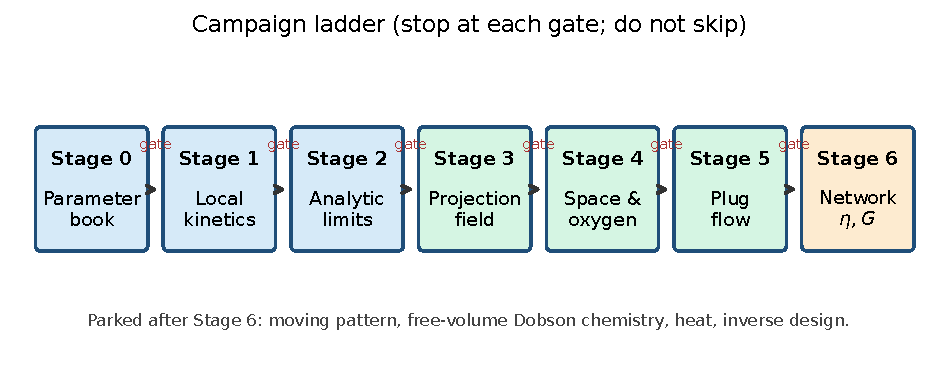
\includegraphics[width=\textwidth]{fig_roadmap_stage_ladder.pdf}
  \caption{Seven active stages.
  Each arrow is a gate: the next box is not opened on engineering success alone.
  After Stage~6, pattern motion, Dobson free-volume chemistry, heat, and inverse design remain parked.}
  \label{fig:ladder}
\end{figure}

\begin{table}[htbp]
\centering
\caption{One-line claim per stage and the literature that owns the claim.}
\label{tab:claims}
\small
\begin{tabularx}{\textwidth}{@{}lp{3.2cm}X@{}}
\toprule
Stage & Claim in one line & Literature owner \\
\midrule
0 & Every coefficient has a provenance or an explicit ``measure'' flag. & Tables in \citet{Montgomery2022,Slutzky2019,Zhu2020,Dobson2024} \\
1 & Prescribed $I(t)$ maps to $p(t)$ with oxygen induction and history dependence. & \citet{Montgomery2022}; reciprocity \citep{Wydra2014,Lin2019} \\
2 & Reduced limits recover algebraic identities, not only curves. & \citet{Slutzky2019} Eq.~3; QSS radicals \citep{Zhu2020}; $R_p$--$I$ exponent \citep{Dobson2024} \\
3 & Bitmap, kernel, and scan produce a conserved surface irradiance. & \citet{Meenakshisundaram2020,Montgomery2022} \\
4 & The same kinetics in space show a wall dead-zone and grayscale blur. & \citet{Montgomery2022,Dendukuri2008} \\
5 & Plug flow recovers a critical speed and $t_{\mathrm{uv}}/t_L$ organisation. & \citet{Slutzky2019} \\
6 & $p$ and $[\mathrm{PEGDA}]_0$ yield $P_{\mathrm{gel}}$, $\eta\le 1$, $G$ below ideal. & \citet{Zhu2020,Macosko1976} \\
\bottomrule
\end{tabularx}
\end{table}

Dimensionless groups decide \emph{which} spatial physics to turn on, not whether the previous stage passed:

\begin{center}
\small
\begin{tabular}{@{}lll@{}}
\toprule
Group & Meaning & If $\mathcal{O}(1)$ or large \\
\midrule
$\beta_{\mathrm{opt}}=AH$ & optical depth & resolve $z$ (Stage~4) \\
$\mathrm{Da}_O$ & oxygen reaction vs diffusion & wall dead-zone \citep{Dendukuri2008} \\
$\Pi_{\mathrm{flow}}$ & photolysis vs advected $\mathrm{O}_2$ & gel/no-gel in flow \citep{Slutzky2019} \\
$\tau_{\mathrm{exp}}=t_{\mathrm{uv}}/t_L$ & pulse vs residence & fiber-length collapse \\
$\Lambda_v=|\mathbf{v}_{\mathrm{pattern}}-\mathbf{u}|/U_*$ & relative pattern motion & do not identify scan with flow \\
$\mathrm{Pe}_i=UH/D_i$ & advection vs diffusion & which species need spatial transport \\
$\chi=\Delta t_{\mathrm{frame}}/t_{\mathrm{chem}}$ & frame vs chemistry & keep discrete DMD frames \\
\bottomrule
\end{tabular}
\end{center}

\section{Cross-cutting reflection protocol}

At the end of \emph{every} stage, before the tag is written, answer these five questions in the journal.
If any answer is ``no'' or ``not applicable because we mixed recipes,'' the tag cannot be \tagmatch, and \tagvalid{} is in doubt.

\begin{enumerate}
  \item \textbf{Which predicate did we compute?}
    Dose, surface $I$, in-resin $I$, $p$, a $2\%$ double-bond threshold \citep{Slutzky2019}, Macosko $P_{\mathrm{gel}}$ \citep{Zhu2020}, $\eta$, or $G$?
    The background note lists the forbidden equivalences; repeating one of them is an automatic \taginvalid.
  \item \textbf{Which paper actually owns this layer?}
    Cite equation or table numbers.
    If the owner is Montgomery and the numbers came from Zhu, the comparison is phenomenological at best.
  \item \textbf{What would make the result unreasonable even if the solver is green?}
    Wrong units of $I$ and $\beta$; $p>1$; gelation at $p=0$ for a dilute precursor that Zhu predicts cannot gel; a ``grayscale'' edge sharper than the optical kernel while diffusion is on; a flow case that gels at infinite $U$.
  \item \textbf{Did equal-dose protocols collapse?}
    If they \emph{do} collapse for a Type~I acrylate with oxygen and bimolecular termination, the constitutive law is suspect \citep{Wydra2014} unless oxygen is absent and $k_t$ is first-order, which must be stated.
  \item \textbf{What is still required?}
    Name the measurement (FTIR $p(t)$, radiometer PSF, oxygen probe, rheology $G$) that would be needed to move \tagvalid{} to \tagmatch.
\end{enumerate}

\paragraph{Fit discipline.}
Parameters are identified in this order, not all at once \citep{Montgomery2022,Dobson2024}:
(i)~photolysis $\beta C_{I,0}$ from initiator decay or very-low conversion;
(ii)~$k_O$ and $C_{O,0}$ from induction time or inhibition thickness;
(iii)~$k_{p0}$ and termination pieces from \emph{several} intensities, including equal-dose pairs;
(iv)~conversion sensitivity $c_p$ from high-conversion slowdown;
(v)~network $C_0$ from gelation versus concentration, independently of the rate fit \citep{Zhu2020}.
A single conversion curve used to fit ten numbers is \taginvalid{} as a parameter inference even if the forward gates pass.

\section{Stage 0 --- Parameter book}

\subsection{Scientific question}
Can every coefficient that will enter later stages be traced to a paper table, a recipe calculation, or an explicit gap labelled \stillreq?

\subsection{What you do}
Transcribe, with units and initiator class:
\begin{itemize}
  \item Montgomery Table~1 (optical attenuation, pixel Gaussian fallback) and the $k_p(p)$, $k_t(p)$ closures \citep{Montgomery2022};
  \item Slutzky Table~2 and the stated $k_d$ window \citep{Slutzky2019};
  \item Zhu's $C_0$, functionality $f=2$, and the statement that PEGDA~$575$ is the hydrogel example \citep{Zhu2020};
  \item Dobson's role as HDDA reference, not as a PEGDA number dump \citep{Dobson2024}.
\end{itemize}
Flag molecular-weight mismatch ($250$ vs $575\,\mathrm{g\,mol^{-1}}$) and Type~I vs Type~II in the same table.
Do not fit anything yet.

\subsection{Success factors}
Provenance is complete; silent defaults are forbidden; SI (or a declared conversion to Montgomery's intensity convention) is written next to $\beta$.

\subsection{Stage gates}
\begin{itemize}
  \item Every parameter has a source column: paper / calculated from recipe / \stillreq.
  \item No row mixes PEGDA~$250$ dry film, PEGDA~$575$ water gel, and HDDA without a chemistry key.
  \item Intensity units for $\beta$ are stated.
\end{itemize}

\subsection{Reasonability and literature}
Reasonable if mass-fraction $\to$ molarity conversions recover $[M]_0$ of order several $\mathrm{mol\,L^{-1}}$ for neat diacrylate and lower for diluted hydrogels, consistent with the papers' recipes.
Unreasonable if one ``PEGDA'' row is used for all three formulations.

\subsection{Tag and stop}
\tagproposed{} until the book exists; then \tagvalid{} for the \emph{bookkeeping} claim only.
Stop. Do not solve ODEs in this stage beyond a unit-smoke if needed to read the file.

\section{Stage 1 --- Local constitutive response}

\subsection{Scientific question}
For a \emph{prescribed} $I(t)$, with no space and no flow, do initiator, radicals, oxygen, and acrylate evolve as a stiff free-radical system with conversion-dependent $k_p$ and $k_t$ \citep{Montgomery2022}?

The balances (Montgomery Eqs.~16--19 with diffusion switched off) are
\begin{align}
  \dot C_I &= -\beta I C_I, \label{eq:CI}\\
  \dot C_R &= m\beta I C_I - 2k_t(p)C_R^2 - k_O C_O C_R, \label{eq:CR}\\
  \dot C_O &= -k_O C_O C_R, \label{eq:CO}\\
  \dot C_M &= -k_p(p)\,C_R C_M, \qquad p=1-C_M/C_{M,0}. \label{eq:CM}
\end{align}
Temperature is held fixed.
Radicals are \emph{not} replaced by a quasi-steady algebraic law at this stage: the stiffness is physical \citep{Montgomery2022,Dobson2024}.

\subsection{What you do}
Integrate~\eqref{eq:CI}--\eqref{eq:CM} for a protocol family: dark; constant $I$; square pulse; two equal-dose pairs $(I_1,t_1)$ and $(I_2,t_2)$ with $I_1 t_1=I_2 t_2$; oxygen-free limit $C_{O,0}=0$.
Export $p(t)$, $C_O(t)$, $R_p(t)$.
Thermal energy stays off.

\subsection{Success factors}
\begin{itemize}
  \item Dark control is dead: no photoinitiator-driven conversion.
  \item An oxygenated sample shows an induction period; the oxygen-free twin does not \citep{Decker1985,Dendukuri2008}.
  \item Equal-dose pairs do \emph{not} collapse in general \citep{Wydra2014,Lin2019}.
  \item High conversion slows as $k_p(p)$ and $k_t(p)$ intend \citep{Montgomery2022,Anseth1994}.
  \item Concentrations stay non-negative; $0\le p\le 1$; $C_I$ and $C_M$ decrease under illumination.
\end{itemize}

\subsection{Stage gates (all required for \tagvalid)}
\begin{center}
\small
\begin{tabular}{@{}p{3.2cm}p{10.2cm}@{}}
\toprule
Gate & Pass criterion \\
\midrule
Dark & $I=0$ $\Rightarrow$ $\Delta p$ below solver tolerance. \\
Positivity & $C_i \ge -10^{-12}\,\mathrm{mol\,m^{-3}}$ without ad-hoc clipping of large negatives. \\
Bounds & $0\le p\le 1$. \\
Monotone PI & $C_I$ nonincreasing when $I>0$. \\
Acrylate balance & $\int R_p\,\mathrm{d}t$ matches $\Delta C_M$ to a stated relative tolerance. \\
Reciprocity & At least one equal-dose pair with $|p_1-p_2|$ at a common dose \emph{not} both consistent with numerical noise. \\
Induction & With $C_{O,0}>0$, $p$ remains near $0$ until $C_O$ has dropped; with $C_{O,0}=0$, that delay vanishes. \\
\bottomrule
\end{tabular}
\end{center}

\subsection{Reasonability and literature}
Compare \emph{shapes} to Montgomery's FTIR conversion-versus-time family \citep{Montgomery2022} and to Wydra's dose plots \citep{Wydra2014}.
Do \emph{not} declare \tagmatch{} unless the formulation (PEGDA~$250$, $0.1\,\mathrm{wt\%}$ Irgacure~819, their $I$ in their units) is the one in the file.
If equal-dose curves collapse, first check that $k_t$ was accidentally made first-order or that oxygen was omitted; that is a constitutive bug, not a discovery.

Quasi-steady radicals~\eqref{eq:qss-ref} are a \emph{diagnostic overlay} in this stage, not a substitute for~\eqref{eq:CR}:
\begin{equation}
  C_R \stackrel{?}{\approx} \sqrt{\frac{m\beta I C_I}{2k_t}}\quad (C_O=0,\ \text{slow transients}).
  \label{eq:qss-ref}
\end{equation}

\subsection{Tag and stop}
\tagsmoke{} after a short protocol set; \tagvalid{} after the full gate table.
\tagmatch{} only against a named Montgomery (or in-house FTIR) series.
Stop. Do not add diffusion here.

\section{Stage 2 --- Analytic and reduced limits}

\subsection{Scientific question}
Does the constitutive law contain the limits the literature actually solved, or only a plausible S-shaped $p(t)$?

\subsection{What you do}
Introduce a \emph{constant-coefficient fork} of~\eqref{eq:CI}--\eqref{eq:CM} (constant $k_p$, $k_t$, $k_O$; still no space).
Test:
\begin{itemize}
  \item Slutzky's algebraic oxygen--monomer relation
    \begin{equation}
      \frac{C_O}{C_{O,0}} = \left(\frac{C_M}{C_{M,0}}\right)^{k_O/k_p}
      \label{eq:slu3}
    \end{equation}
    which follows from dividing the $M$ and $\mathrm{O}_2$ balances when those two rates dominate \citep{Slutzky2019};
  \item oxygen-free QSS radicals against~\eqref{eq:qss-ref} after the fast transient \citep{Zhu2020};
  \item qualitative $R_p$ versus $I$: exponent near $1/2$ when bimolecular termination wins, nearer $1$ when oxygen makes radical loss pseudo-first-order \citep{Dobson2024}.
\end{itemize}
The last test is \emph{not} a demand to reproduce Dobson's HDDA numbers.

\subsection{Success factors}
Identities hold to a pre-declared \texttt{rtol}/\texttt{atol}.
The $R_p$--$I$ exponent moves in the direction Dobson describes when $C_{O,0}$ is raised at fixed low $I$.

\subsection{Stage gates}
\begin{itemize}
  \item Equation~\eqref{eq:slu3} on the constant-rate fork: maximum relative residual below the declared band (e.g.\ $10^{-4}$ away from $C_M\to 0$).
  \item QSS residual $|C_R-\sqrt{R_i/2k_t}|/C_R$ small after a stated number of radical times, for $C_{O,0}=0$.
  \item Full conversion-dependent model is \emph{not} required to satisfy~\eqref{eq:slu3}; the journal must say so, or the test is meaningless.
\end{itemize}

\subsection{Reasonability and literature}
This is the campaign's manufactured-solution analogue: we test the algebra the papers derived, not their figures.
Failure here means the right-hand side was transcribed wrongly.
Do not ``fix'' $k_t$ to make~\eqref{eq:slu3} hold in the conversion-dependent model.

\subsection{Tag and stop}
\tagvalid{} if identities pass.
No \tagmatch{} is available at this stage (no experiment yet).
Stop.

\section{Stage 3 --- Projection engine}

\subsection{Scientific question}
Given a bitmap, a spatial kernel, and optional scan motion, what is the surface irradiance $I_\perp(x,y,t)$, and is energy accounted for \citep{Meenakshisundaram2020,Montgomery2022}?

This stage has \emph{no chemistry}.

\subsection{What you do}
\begin{itemize}
  \item Implement superposition of pixel kernels. Montgomery's Gaussian (their Eq.~7) is the fallback \citep{Montgomery2022}.
  \item Allow a measured, non-Gaussian kernel as the scientifically preferred input \citep{Meenakshisundaram2020}.
  \item Accumulate dose $E_\perp=\int I_\perp\,\mathrm{d}t$ under a scan whose frame period is projected pitch divided by scan speed \citep{Meenakshisundaram2020}.
  \item Optionally overlay a Jacobs $C_d=D_p\ln(E/E_c)$ field, labelled \textbf{diagnostic, not state} \citep{Jacobs1992book}.
\end{itemize}

\subsection{Success factors}
A single pixel's integrated power matches the commanded pixel power.
Overlapping Gaussians produce the qualitative bleed of Montgomery's Fig.~3.
Scan: if dwell $\propto 1/v$, peak $E_\perp$ is approximately $v$-independent; if not, the journal explains why (frame discreteness, $\chi$ not small).

\subsection{Stage gates}
\begin{itemize}
  \item Power conservation of one pixel to a stated relative error.
  \item Ten-pixel overlap: irradiance at a commanded edge is not a top-hat (bleed exists).
  \item Dark bitmap $\Rightarrow$ $I_\perp=0$.
  \item Chemistry disabled: no $p$ is reported as a Stage~3 result.
\end{itemize}

\subsection{Reasonability and literature}
Compare kernel shape to Meenakshisundaram's measured profiles (non-Gaussian, possible flat top).
If a Gaussian is used, the journal must say the projection error relative to a measured PSF is \stillreq.
Do not compare printed widths from Jacobs overlays to Montgomery conversion fields and call it validation.

\subsection{Tag and stop}
\tagvalid{} on conservation and bleed.
\tagmatch{} only if a camera/radiometer map of \emph{this} projector is used.
Stop. Do not couple attenuation yet.

\section{Stage 4 --- Spatial reaction--diffusion and light}

\subsection{Scientific question}
If the Stage~1 right-hand side is evaluated in space, with Beer--Lambert attenuation and conversion-dependent diffusivities, do we obtain (i)~depth structure and (ii)~lateral blur beyond the optical kernel \citep{Montgomery2022}?
As a variant: does an oxygen Dirichlet or permeable wall create a dead zone \citep{Dendukuri2008}?

The optical reduction is
\begin{equation}
  \frac{\partial I}{\partial z}+A(\mathbf{x},t)I=0,\qquad
  A=\alpha_I C_I + p A_{\mathrm{poly}}+(1-p)A_{\mathrm{mon}}+A_{\mathrm{abs}},
  \label{eq:beer}
\end{equation}
following \citet{Montgomery2022}.
Species follow
\begin{equation}
  \partial_t C_i = \nabla\cdot\bigl(D_i(p)\nabla C_i\bigr)+R_i,
\end{equation}
with the same $R_i$ as Stage~1.
First geometry: one-dimensional $z$.
Second: an $x$--$z$ grayscale strip.
Not three dimensions.

Two boundary-condition variants must be labelled:
\begin{description}
  \item[Sealed slides] no-flux, Montgomery's FTIR cell.
  \item[Oxygen wall] fixed $C_O$ or permeable flux, Dendukuri/CLIP-type dead zone \citep{Dendukuri2008,Tumbleston2015}.
\end{description}
They are different experiments.

\subsection{What you do}
Method of lines in space; local stiff reaction as in Stage~1.
Harmonic liquid--solid $D_i(p)$ as in Montgomery, unless a later stage replaces it by Dobson free volume (parked).
Run: dark box; uniform illumination, sealed; uniform illumination, oxygen wall; grayscale step $G_0|G_{80}$.

\subsection{Success factors}
\begin{itemize}
  \item Dark sealed box conserves $\int C_M$.
  \item Optically thick $\beta_{\mathrm{opt}}\gtrsim 1$ produces a conversion front, not a uniform $p(z)$ \citep{Cabral2005,Zhu2020,Montgomery2022}.
  \item Oxygen wall: a layer of near-zero $p$ at the boundary; sealed slides: much weaker surface inhibition.
  \item Grayscale: chemical transition width $>$ optical $\sigma$ when radical or monomer diffusion is on \citep{Montgomery2022}.
\end{itemize}

\subsection{Stage gates}
\begin{itemize}
  \item Conservation (sealed, dark) to a stated mass residual.
  \item Manufactured diffusion-only problem (no reaction) recovers a known Gaussian spread or similar.
  \item Fourier/CFL (or implicit stability) documented; no grid-scale ringing in $C_R$ that changes $p$ by more than the gate band under refinement.
  \item Grayscale width test as above, with diffusion on versus off.
  \item The Stage~1 ODE at one collocation point with the local $I(t)$ extracted from the field agrees with the spatial cell (same RHS).
\end{itemize}

\subsection{Reasonability and literature}
Phenomenology: Montgomery's overcure and edge blur; Dendukuri's inhibition layer.
\tagmatch{} requires their geometry, absorber loading, and PEGDA~$250$ recipe, or an in-house film with measured $I(z=0)$.
Unreasonable: a dead zone in a sealed, deoxygenated film; or no dead zone against air/PDMS when $\mathrm{Da}_O$ is large.

\subsection{Tag and stop}
\tagvalid{} on conservation, MMS, and the two qualitative structures (front, blur or dead zone).
Stop. Do not add flow.

\section{Stage 5 --- Plug-flow benchmark}

\subsection{Scientific question}
If material is carried at uniform speed $U$ through a fixed illumination window of length $L$, do initiator, radicals, monomer, and oxygen follow Slutzky's steady balances, and does a critical speed separate gel from no-gel \citep{Slutzky2019}?

\begin{equation}
  U\frac{\mathrm{d}C_i}{\mathrm{d}x}=R_i(C,I(x)),\qquad I(x)>0\ \text{only on }[0,L].
\end{equation}
This is the Lagrangian twin of Stage~1 under $t=x/U$ \emph{if} diffusion is negligible, as Slutzky argue for their jet ($\sqrt{Dt}\ll w_1$).

Use \emph{their} operational gel predicate $C_M/C_{M,0}=0.98$ when comparing to their fiber onset---and write that sentence explicitly, because it is not Zhu's $P_{\mathrm{gel}}$ \citep{Zhu2020,Slutzky2019}.

\subsection{What you do}
Integrate in $x$ with their Table~2 as a labelled parameter set.
Sweep $U$ and $I$.
Form $\tau_{\mathrm{exp}}=t_{\mathrm{uv}}/t_L$ for pulsed cases.
Do not enable wall oxygen diffusion unless a variant is named ``not Slutzky's jet.''

\subsection{Success factors}
\begin{itemize}
  \item $U\to\infty$: negligible conversion in the window.
  \item Small $U$, long $t_{\mathrm{uv}}$: the $2\%$ threshold is crossed.
  \item $U_c$ increases with $I$ and with $[\mathrm{PI}]_0/[\mathrm{O}_2]_0$ in the sense of their scaling.
  \item Fiber-length organisation against $t_{\mathrm{uv}}/t_L$ is monotonic in the uniform-fiber regime they describe.
\end{itemize}

\subsection{Stage gates}
\begin{itemize}
  \item The two limits (fast flow / slow flow) as above.
  \item Constant-rate fork still satisfies~\eqref{eq:slu3} along $x$.
  \item Gel predicate documented: $2\%$ vs Macosko, never mixed in one figure without a dual axis and a caption warning.
\end{itemize}

\subsection{Reasonability and literature}
\tagmatch{} is allowed only against Slutzky Table~2 and their figures, with PEGDA~$575$ jet chemistry---not Montgomery thin-film rates.
Unreasonable: gelation that is independent of $[\mathrm{O}_2]_0$ while $k_O$ is large; or a critical speed that decreases as $I$ increases.

\subsection{Tag and stop}
Qualitative scaling: \tagvalid.
Their numbers: \tagmatch{} if within a pre-declared band (they report tight length statistics; do not demand $2.9\%$ dimensional error from a different paper).
Stop.

\section{Stage 6 --- Network post-processor}

\subsection{Scientific question}
Given $p$ and $[\mathrm{PEGDA}]_0$, when does a sample-spanning network appear, and what elastically active fraction $\eta$ and phantom modulus $G$ follow, including loops \citep{Zhu2020,Macosko1976,Miller1976}?

\begin{equation}
  \theta=\frac{[\mathrm{PEGDA}]_0}{[\mathrm{PEGDA}]_0+2C_0},\qquad
  P_{\mathrm{gel}}=\frac{1-\theta}{2\theta}=\frac{C_0}{[\mathrm{PEGDA}]_0},
\end{equation}
\begin{equation}
  G=\eta N_A [\mathrm{PEGDA}]_0 k_B T,\qquad \eta\le 1.
\end{equation}
This stage does \emph{not} advance $C_I$ or $C_R$.
It maps fields from Stages~1, 4, or 5.

\subsection{What you do}
Implement the recursive probabilities as in Zhu (pre- and post-gel).
Sweep $[\mathrm{PEGDA}]_0$ through $C_0$.
Apply $\eta(p)$ to a conversion field from an earlier stage without refitting $k_p$.

\subsection{Success factors}
\begin{itemize}
  \item $[\mathrm{PEGDA}]_0\le C_0$ $\Rightarrow$ no gel at $p=1$.
  \item $\theta\to 1$ $\Rightarrow$ $P_{\mathrm{gel}}\to 0$.
  \item $G < G_{\mathrm{ideal}}$ when loops are allowed; $\eta=p^2$ recovered in the no-loop limit they state.
\end{itemize}

\subsection{Stage gates}
The three bullets above as tests.
Chemistry flag: eosin~Y bleaching ODEs are off unless a Type~II branch is explicitly selected.
No use of $G$ to retune Stage~1 rates.

\subsection{Reasonability and literature}
Compare gel-versus-concentration and $G$ versus $p$ to Zhu's rheology/indentation \emph{only} for their eosin~Y PEGDA~$575$ water system.
Applying $\eta$ to a Montgomery Type~I conversion field is a \emph{hypothetical} network map: allowed if labelled, not \tagmatch{} to Zhu's figures.

\subsection{Tag and stop}
Algebraic limits: \tagvalid.
Zhu's mechanical data: \tagmatch{} only on their formulation.
Park FEM, swelling, and inverse design.

\section{Parked stages (not opened by this note)}

\begin{tabularx}{\textwidth}{@{}lXl@{}}
\toprule
Item & Reopen when & Needed \\
\midrule
Moving $\mathbf{v}_{\mathrm{pattern}}\neq 0$ & Stage~3 \tagvalid{} and $\Lambda_v$ not $\approx 0$ in the experiment & scan kinematics \\
Eulerian--Lagrangian markers & Stages~4--5 \tagvalid & $\mathbf{u}(\mathbf{x})$ \\
Dobson free-volume / chain-length $k_t$ & equal-dose tests fail after a correct Stage~1 transcription & two-intensity FTIR \\
Energy equation & isothermal $p(t)$ systematically wrong vs measured $T$ & $\Delta H_p$, $h$ \\
Inverse DMD & Stage~4 grayscale widths \tagmatch{} & target $\eta$ maps \\
\bottomrule
\end{tabularx}

\section{What this campaign will refuse to cite}

\begin{itemize}
  \item Jacobs depth as conversion, gelation, or modulus.
  \item Montgomery coefficients as universal PEGDA constants.
  \item A $2\%$ double-bond ``gel'' plotted as Zhu's $P_{\mathrm{gel}}$ without a caption.
  \item Equal-dose collapse presented as a virtue of the acrylate Type~I model.
  \item Any Stage~$n$ figure used as evidence for Stage~$n+1$'s claim.
\end{itemize}

\section{Immediate next action}

Open \textbf{Stage~0} (parameter book) and \textbf{Stage~1} (local constitutive response) only.
Do not scaffold Stages~3--6 until Stage~1 is \tagvalid{} and Stage~2 identities have been attempted.

All claims in this document remain \tagproposed{} until those gates exist in the laboratory record.

\bibliographystyle{plainnat}
\bibliography{background_photopolymerization}

\end{document}
